\documentclass{article}
\usepackage{graphicx}
\usepackage[export]{adjustbox}
\usepackage{tabularx}  %better tables
\usepackage{hyperref}

\title{Homework 3 CSCI 451}
\author{Nicholas Rust}
\date{due: 11 October 2019}

\begin{document}
\maketitle

\section{Exercise 1 (textbook section 3.8, pg 82)}
\begin{verbatim}
a. gat
		
S = acgatca
T =   gattact
X = aagatgt
\end{verbatim}
b. An algorithm that creates a suffix tree for all three of the strings overlaid, then finds the branches with one leaf from every string, and follows that branch back up to the lowest common ancestor, the deepest lowest common ancestor will be the longest string. The string available from the LCA to the root will be the longest common substring. O($|S| * |T| * |X|$) O($|S| + |T| + |X|$)\\
c.  An algorithm that creates a suffix tree for all three of the strings overlaid, then finds branches with one leaf from every string, and follows that branch back up to the lowest common ancestor. The string available from the LCA to the root will be a common substring, then compare each of these to find the longest or multiple longest. O($|S| * |T| * |X|$)

\section{Exercise 2 (textbook section 3.8, pg 84)}
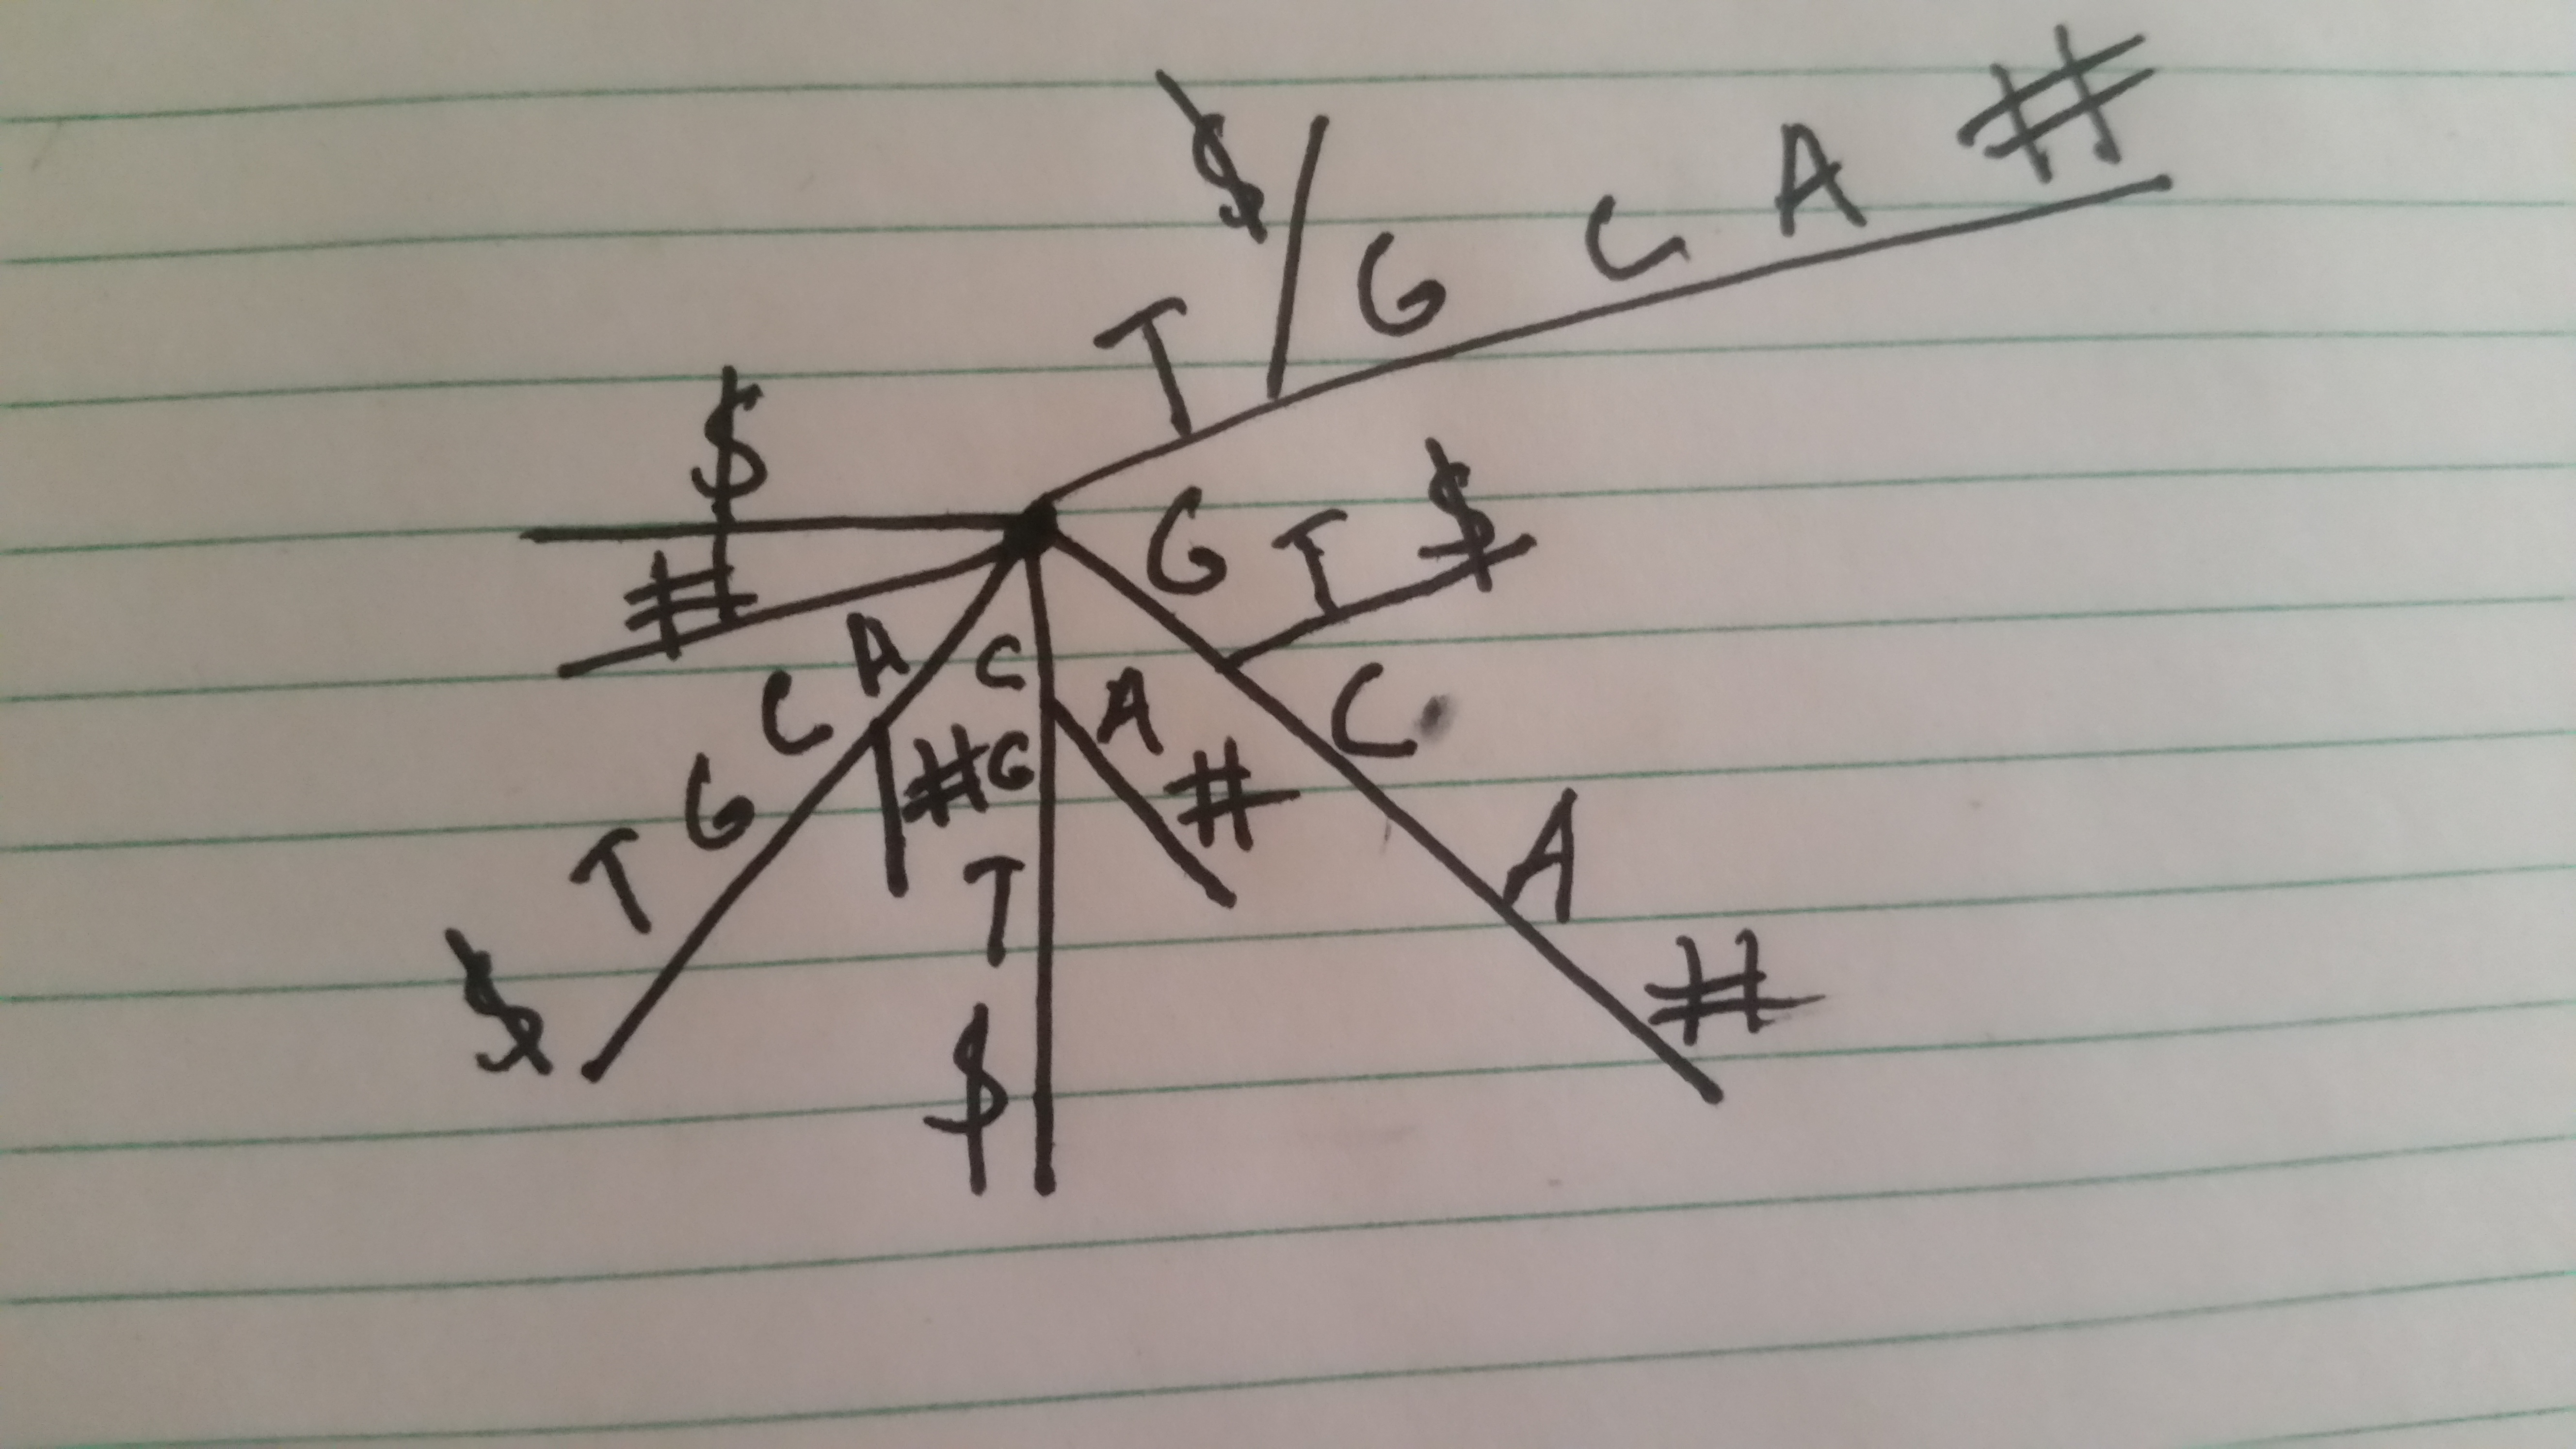
\includegraphics[width=1.75\textwidth,center]{problem2.jpg}

\section{Exercise 3 (textbook section 3.8, pg 84)}
Create a suffix tree O($|S|$). Compare the pattern to the tree and find the branch it matches, follow that until the end of the pattern, this will give the location of every occurrence of the pattern. This will have a hamming distance of 0 and time complexity of O($|P|$). In order to accommodate a hamming distance of 1, and therefore the O($|P|^2$) time complexity, we would have to test every position in P as any other character, allowing for 1 modification.

\pagebreak

\section{Exercise 19 (textbook section 3.8, pg 86)}
a. False. If alpha is after an inner node, there could conceivably be a repeat of just the portion of alpha which is beta that comes after another separate string. As shown above. On page 67 there is an example of a tree where if we take the path to leaf node 1 and call that alpha = cag\$, beta = ca. We can see directly above the leaf node 1 is the path beta as an inner node.
\begin{figure}
    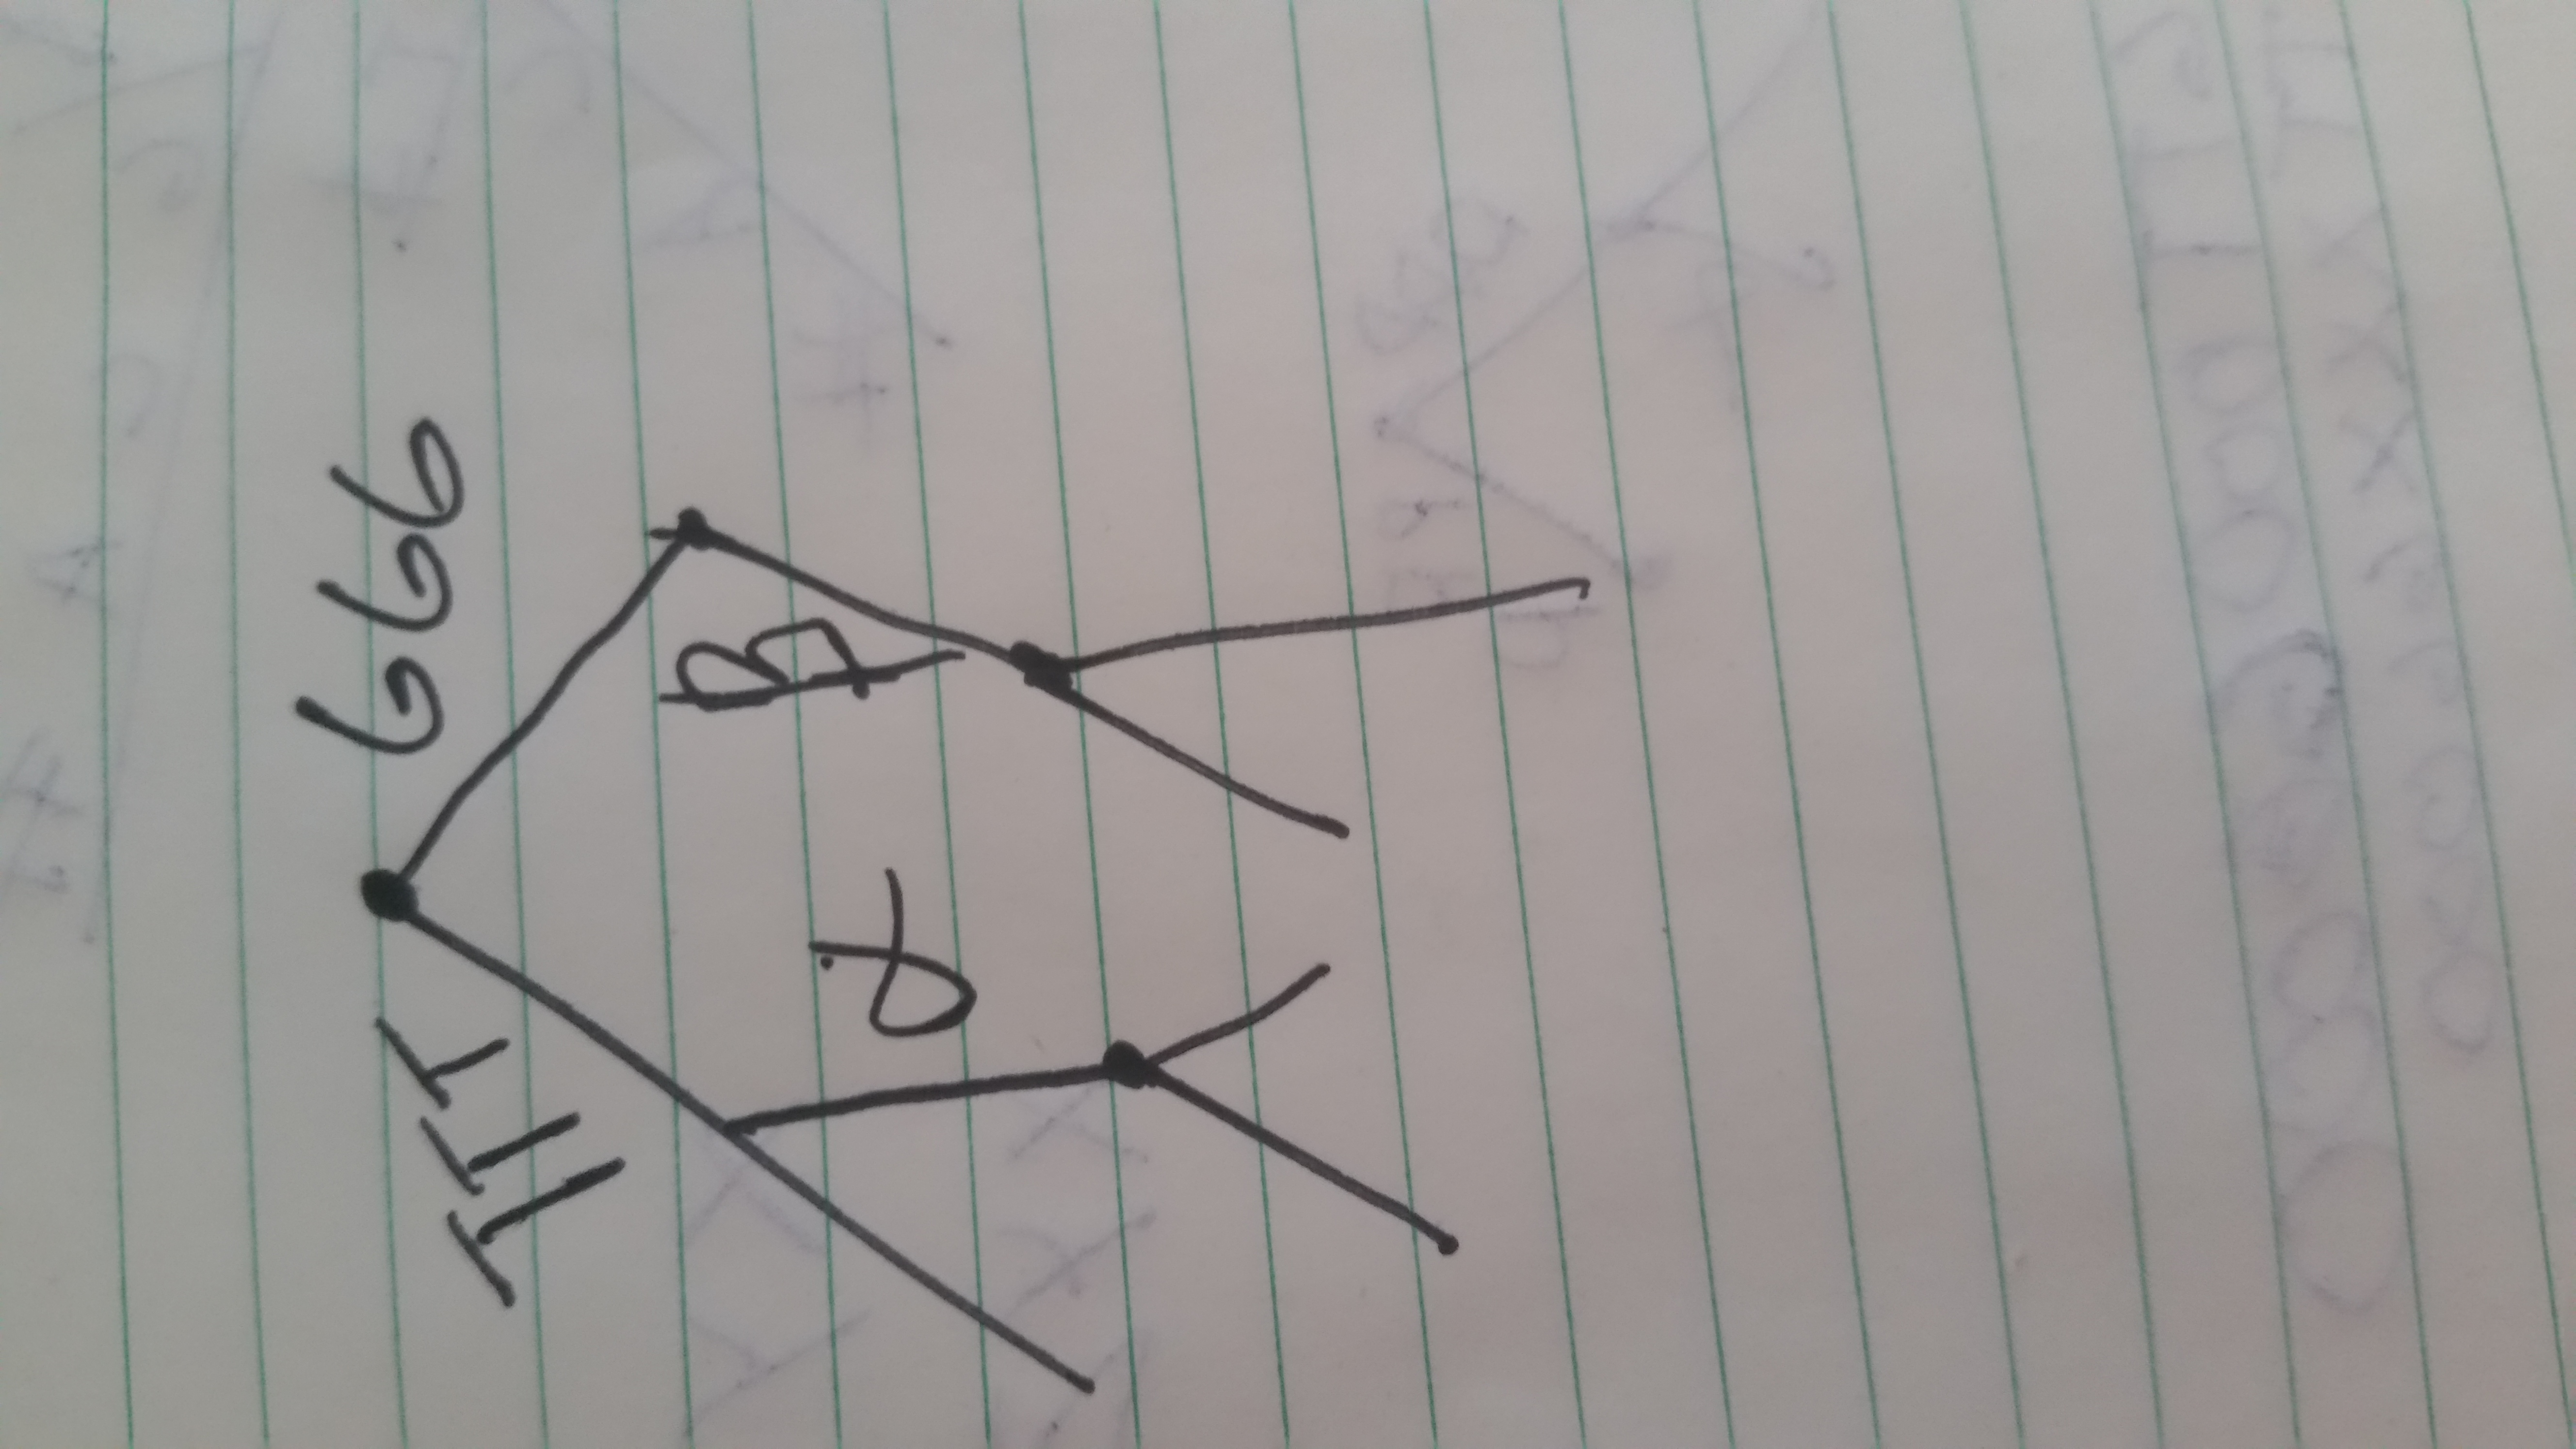
\includegraphics[width=1.75\textwidth,center]{problem19.jpg}
    \caption{Exercise 19 (a)}
\end{figure}\\
b. True. This is the idea that suffix links are based on. Where every substring u will have all other suffixes of it somewhere else in the tree.

\section{Exercise 20 (textbook section 3.8, pg 86)}
\bgroup
\def\arraystretch{1.5}%
\begin{tabularx}{8cm}{| X | X | X | X |}
  \hline
  \textbf{i} & \textbf{SA[i]} & \textbf{BW[i]} & \textbf{Suffix}\\
  \hline
  1 & 8 & a  & \$		\\
  2 & 7 & g  & a\$		\\
  3 & 1 & \$ & acgtcga\$\\
  4 & 5 & t  & cga\$	\\ 
  5 & 2 & a  & cgtcga\$ \\
  6 & 6 & c  & ga\$		\\
  7 & 3 & c  & gtcga\$	\\
  8 & 4 & g  & tcga\$	\\
  \hline
\end{tabularx}
\egroup

\vspace{.5cm}

Finding pattern cg in suffix array.

\bgroup
\def\arraystretch{1.5}%
\begin{tabularx}{8cm}{| X | X |}
  \hline
  \textbf{i} & \textbf{Suffix}\\
  \hline
  1 & \$		\\
  2 & a\$		\\
  3 & acgtcga\$ \\
  4 & cga\$		\\ 
  Check here -- Match & cgtcga\$ \\
  6 & ga\$		\\
  7 & gtcga\$	\\
  8 & tcga\$	\\
  \hline
\end{tabularx}
\egroup

\vspace{.5cm}

\bgroup
\def\arraystretch{1.5}%
\begin{tabularx}{8cm}{| X | X |}
  \hline
  \textbf{i} & \textbf{Suffix}\\
  \hline
  1 & \$		\\
  2 & a\$		\\
  Check here -- Mismatch & acgtcga\$ \\
  4 & cga\$		\\ 
  5 Checked -- Match & cgtcga\$ \\
  6 & ga\$		\\
  Check here -- Mismatch & gtcga\$	\\
  8 & tcga\$	\\
  \hline
\end{tabularx}
\egroup

\vspace{.5cm}

\bgroup
\def\arraystretch{1.5}%
\begin{tabularx}{8cm}{| X | X |}
  \hline
  \textbf{i} & \textbf{Suffix}\\
  \hline
  1 & \$		\\
  2 & a\$		\\
  3 Checked -- Mismatch & acgtcga\$ \\
  Check here -- Match & cga\$		\\ 
  5 Checked -- Match & cgtcga\$ \\
  Check here -- Mismatch & ga\$		\\
  7 Checked -- Mismatch & gtcga\$	\\
  8 & tcga\$	\\
  \hline
\end{tabularx}
\egroup

\vspace{.5cm}

\bgroup
\def\arraystretch{1.5}%
\begin{tabularx}{8cm}{| X | X |}
  \hline
  \textbf{i} & \textbf{Suffix}\\
  \hline
  1 & \$		\\
  2 & a\$		\\
  3 Checked -- Mismatch & acgtcga\$ \\
  4 Checked -- Match & cga\$		\\ 
  5 Checked -- Match & cgtcga\$ \\
  6 Checked -- Mismatch & ga\$		\\
  7 Checked -- Mismatch & gtcga\$	\\
  8 & tcga\$	\\
  \hline
\end{tabularx}
\egroup

\vspace{.5cm}
Matches found at SA[5] and SA[2]

\section{Paper}

Genome Majority Vote Improves Gene Predictions

\vspace{.2cm}

Cat Search:

\vspace{.2cm}

\url{https://msu-primo.hosted.exlibrisgroup.com/primo-explore/fulldisplay?docid=TN_plos10.1371%2Fjournal.pcbi.1002284&context=PC&vid=01TRAILS_MSU&lang=en_US&search_scope=01TRAILS_MSU&adaptor=primo_central_multiple_fe&tab=everything&query=any,contains,computational%20biology%20gene&offset=0}

\vspace{.2cm}

PDF:

\vspace{.2cm}

\url{https://journals.plos.org/ploscompbiol/article/file?id=10.1371\%2Fjournal.pcbi.1002284&type=printable}

\end{document}